\usepackage{xcolor}
\usepackage{afterpage}
\usepackage{float}
\usepackage{caption}
\usepackage{tabularx}
\usepackage{pifont,mdframed}
\usepackage[bottom]{footmisc}
\usepackage{listings}
\usepackage{multicol}

\lstset{
	columns=flexible,
	basicstyle=\small\ttfamily,
	mathescape=true,
	escapeinside=||
}

\createsection{\Circuits}{Circuiti}
\createsection{\InputFormat}{Formato dell'input}
\createsection{\OutputFormat}{Formato dell'output}

\renewcommand{\inputfile}{\texttt{stdin}}
\renewcommand{\outputfile}{\texttt{stdout}}
\makeatletter
\renewcommand{\this@inputfilename}{\texttt{input}}
\renewcommand{\this@outputfilename}{\texttt{output}}
\makeatother

\newenvironment{warning}
  {\par\begin{mdframed}[linewidth=2pt,linecolor=gray]%
    \begin{list}{}{\leftmargin=1cm
                   \labelwidth=\leftmargin}\item[\Large\ding{43}]}
  {\end{list}\end{mdframed}\par}
\newenvironment{danger}
{\par\begin{mdframed}[linewidth=2pt,linecolor=red!60!yellow,backgroundcolor=red!20!white]%
		\begin{list}{}{\leftmargin=1cm
				\labelwidth=\leftmargin}\item[\Large\ding{45}]}
		{\end{list}\end{mdframed}\par}

% % % % % % % % % % % % % % % % % % % % % % % % % % % % % % % % % % % % % % % % % % %
% % % % % % % % % % % % % % % % % % % % % % % % % % % % % % % % % % % % % % % % % % %

Il server delle Olimpiadi Italiane di Informatica si è guastato proprio il
giorno della finale nazionale! Ce la faranno i sistemisti molisani a riportarlo
online prima dell'inizio della gara?

Dopo un'attenta analisi, è venuto fuori che ci sono dei circuiti bruciati da sostituire.
Fortunatamente, nel laboratorio del Marconi ci sono un saldatore ed
abbastanza componenti per ricostruire da zero i circuiti mancanti.
Dario, il tutor smanettone, si è offerto di eseguire la riparazione.
Quello che gli manca però è il progetto (schema elettrico) dei circuiti.
Aiuta Dario a progettare lo schema dei circuiti mancanti!

Un circuito legge un array di $N$ interi
tramite i \emph{registri di input} \texttt{in[$i$]} ($0 \le i < N$),
e può scrivere il risultato sui \emph{registri di output} \texttt{out[$i$]}.
Ci sono tre tipi di circuiti da sostituire, che devono realizzare le seguenti operazioni.

\begin{table}[H]
	\begin{tabularx}{\textwidth}{l|X}
		\textbf{Somma} &
		Scrivere su \texttt{out[$0$]} la somma degli $N$ interi in input.\\[5pt]
		\hline \\[-10pt]
		\textbf{Prefissi} &
		Scrivere sui registri di output l'array delle somme prefisse, definito come
		$\texttt{out[$i$]} = \texttt{in[$0$]} + \cdots + \texttt{in[$i$]}$ con $0 \le i < N$.\\[5pt]
		\hline \\[-10pt]
		\textbf{Massimo sottoarray} &
		Scrivere su \texttt{out[$0$]} il più grande numero ottenibile come somma di elementi consecutivi dell'array di input
		(ovvero, che si possa scrivere come $\texttt{in[$i$]} + \cdots + \texttt{in[$j$]}$ con $0 \le i \le j < N$). Anche il vettore
		vuoto vale come sottoarray, per cui il risultato di questa operazione è sempre almeno $0$.
	\end{tabularx}
\end{table}

Oltre ai registri di input e output,
un circuito può contenere \emph{registri intermedi}.
Inoltre esistono dei registri speciali che forniscono delle
\emph{costanti} che possono essere usate come ingresso per gli altri componenti.

Un circuito è formato da diversi \emph{componenti}, come esemplificato in Figura 1.
Ogni componente è collegata a due registri di ingresso e un registro di uscita,
e implementa una fra le seguenti operazioni matematiche:
somma (\texttt{+}), differenza (\texttt{-}) e massimo (\texttt{max}).
Appena vengono scritti i valori di entrambi i registri di ingresso,
il componente effettua il calcolo e, dopo un ciclo di clock,
scrive il risultato dell'operazione scelta sul suo registro di uscita.
Il registro di uscita può a sua volta essere collegato (come registro di ingresso) ad uno o più componenti, che eseguiranno il calcolo appena avranno disponibili entrambi i loro ingressi e così via.

I registri di input possono essere usati solo come ingressi,
mentre i registri intermedi e i registri di output
sono uscite di \textbf{esattamente una} componente.
Il calcolo termina quando tutti i registri sono stati scritti.

\begin{figure}[t]%
	\centering\includegraphics[scale=1]{asy_circuiti/figs.pdf}
	\caption{Esempio di realizzazione della formula:
	\[
	\texttt{out[$0$]} = \max(\texttt{in[$0$]} + \texttt{in[$1$]} + 5 + \texttt{in[$3$]},
	(5 + \texttt{in[$3$]}) - (\texttt{in[$3$]} + \texttt{in[$4$]})) + \texttt{in[$5$]}
	\]} \label{fig}
\end{figure}

Per ciascun circuito che deve essere progettato,
conosci il tipo di circuito (somma, prefissi o massimo sottoarray),
il numero $N$ di registri di input,
e il tempo di calcolo $C$ desiderato (espresso in cicli di clock).

Aiuta Dario a progettare tutti i circuiti che mancano,
in modo tale che funzionino \textbf{qualunque siano i dati in ingresso},
e che il loro tempo di calcolo sia il più possibile vicino a quello desiderato.
Cerca inoltre di non usare troppi componenti: ogni circuito viene con
$1100$ componenti in regalo, ma ogni ulteriore componente va
comprato!

\pagebreak
I circuiti che dovrai progettare sono i seguenti:
\begin{center}
	\begin{tabular}{c|c|c|c}
		\textbf{Input} & \textbf{Tipo} & $N$ & $C$ \\[5pt]
		\hline \\[-10pt]
		\texttt{input000.txt} & Somma & 7 & 3 \\
		\texttt{input001.txt} & Somma & 256 & 8 \\
		\texttt{input002.txt} & Somma & 1093 & 11 \\[5pt]
		\hline \\[-10pt]
		\texttt{input003.txt} & Prefissi & 7 & 5 \\
		\texttt{input004.txt} & Prefissi & 128 & 13 \\
		\texttt{input005.txt} & Prefissi & 371 & 15 \\[5pt]
		\hline \\[-10pt]
		\texttt{input006.txt} & Massimo sottoarray & 7 & 15 \\
		\texttt{input007.txt} & Massimo sottoarray & 64 & 31 \\
		\texttt{input008.txt} & Massimo sottoarray & 110 & 35 \\
		\texttt{input009.txt} & Massimo sottoarray & 124 & 35 \\
	\end{tabular}
\end{center}

% % % % % % % % % % % % % % % % % % % % % % % % % % % % % % % % % % % % % % % % % % %
% % % % % % % % % % % % % % % % % % % % % % % % % % % % % % % % % % % % % % % % % % %

\InputFormat

I circuiti da progettare sono riportati nei file di input come nella tabella precedente. Ogni file consiste in tre interi $T$, $N$ e $C$ dove $T$ indica il tipo di circuito da realizzare ($1$ per la somma, $2$ per i prefissi, $3$ per il massimo sottoarray).

% % % % % % % % % % % % % % % % % % % % % % % % % % % % % % % % % % % % % % % % % % %
% % % % % % % % % % % % % % % % % % % % % % % % % % % % % % % % % % % % % % % % % % %

\OutputFormat

Il circuito da te progettato va descritto sotto forma di componenti e corrispettive connessioni. Ogni riga del file di output rappresenta un componente, secondo uno dei tre seguenti formati possibili:
\[
C[k] = A[i]\ \texttt{op}\ B[j] \qquad C[k] = i\ \texttt{op}\ B[j] \qquad C[k] = A[i]\ \texttt{op}\ j
\]
in cui:
\begin{itemize}
	\item $A$, $B$ e $C$ sono nomi di array. Questi nomi possono essere composti da massimo 50 caratteri alfanumerici (maiuscoli o minuscoli), e non devono cominciare con una cifra.
	\item $i$, $j$, $k$ sono costanti intere positive, che devono stare in un intero a 32 bit con segno.
	\item \texttt{op} è un operatore a scelta fra \texttt{+}, \texttt{-} o \texttt{max}.
\end{itemize}
Tale riga definisce un componente che ha $A[i]$ e $B[j]$ come registri di ingresso (o le costanti $i$ e $j$ rispettivamente), $C[k]$ come registro di uscita, e implementa l'operazione \texttt{op}.

I due array speciali \texttt{in} e \texttt{out} indicano rispettivamente i registri di input e output. È possibile usare a piacere altri array come registri intermedi. Tuttavia, prima di definire un componente che usa un certo registro intermedio come ingresso, è necessario che un componente \textbf{precedentemente definito} nel file lo abbia come uscita.

% % % % % % % % % % % % % % % % % % % % % % % % % % % % % % % % % % % % % % % % % % %
% % % % % % % % % % % % % % % % % % % % % % % % % % % % % % % % % % % % % % % % % % %


\Scoring

I file di output inviati verranno controllati e valutati da un correttore il quale
verificherà la correttezza del formato e la correttezza del circuito realizzato,
e assegnerà a ciascuno di essi un punteggio da $0$ a $10$.

Se il file inviato non è corretto riceverà punteggio $0$. Altrimenti, gli verrà assegnato un punteggio $P$ secondo la seguente formula:
\[
	P = 10 \cdot \min \left\{1, \frac{C_\text{richiesto}}{C_\text{ottenuto}}\right\} \cdot \min \left\{1, \frac{1100}{S_\text{ottenuto}}\right\}
\]
dove $C_\text{ottenuto}$ è il tempo di calcolo del tuo circuito, e $S_\text{ottenuto}$ è il suo numero di componenti.
Nota che il tuo file riceverà punteggio pieno $10$ se e solo se $C_\text{ottenuto}$ è pari o inferiore a $C_\text{richiesto}$ e $S_\text{ottenuto}$ è pari o inferiore a $1100$.

% % % % % % % % % % % % % % % % % % % % % % % % % % % % % % % % % % % % % % % % % % %
% % % % % % % % % % % % % % % % % % % % % % % % % % % % % % % % % % % % % % % % % % %


\Examples

Lo schema disegnato nel testo corrisponde al seguente file di output:
\begin{lstlisting}
add[0] = in[0] + in[1]
add[1] = 5 + in[3]
add[2] = in[3] + in[4]
add[3] = add[0] + add[1]
add[4] = add[1] - add[2]
m[7] = add[3] max add[4]
out[0] = m[7] + in[5]
\end{lstlisting}
anche se non è la soluzione di nessun input valido. La visualizzazione di questo output, \textbf{o di qualunque altro da te prodotto}, può essere ottenuta cliccando sull'icona di un circuito presente nella barra delle applicazioni alla sinistra del tuo schermo. L'applicazione corrispondente ti chiederà di selezionare un file e ti mostrerà il PDF ad esso corrispondente (contenente il disegno di un circuito o eventuali errori presenti nel file). Il visualizzatore posiziona i componenti corrispondenti allo stesso ciclo di clock $t$ nell'ordine in cui sono riportati nel file, da sinistra verso destra.

Possibili soluzioni di input, diversi da quelli che dovrai progettare, sono presentati di seguito.
\begin{example}
\exmpfile{circuiti.input0.txt}{circuiti.output0.txt}%
\exmpfile{circuiti.input1.txt}{circuiti.output1.txt}%
\exmpfile{circuiti.input2.txt}{circuiti.output2.txt}%
\end{example}

% % % % % % % % % % % % % % % % % % % % % % % % % % % % % % % % % % % % % % % % % % %
% % % % % % % % % % % % % % % % % % % % % % % % % % % % % % % % % % % % % % % % % % %


\Explanation

Nel \textbf{primo caso di esempio} si tratta di sommare 3 interi in input, per esempio,
se l'input fosse $\texttt{in[0]} = -10$, $\texttt{in[1]} = 3$, $\texttt{in[2]} = 5$ allora
il valore di \texttt{temp[0]} sarà $-7$ e \texttt{out[0]} varrà $-2$. Le due operazioni devono
essere eseguite una dopo l'altra, impiegando quindi due cicli di clock a produrre il risultato.
\begin{center}
	\vspace{-5pt}
	\includegraphics[scale=1]{asy_circuiti/fig0.pdf}
	\vspace{-5pt}
\end{center}
Nel \textbf{secondo caso di esempio}, dato lo stesso input del caso precedente, l'output
varrà: $\texttt{out[0]} = -10$, $\texttt{out[1]} = -7$, $\texttt{out[2]} = -2$. Nota che
il terzo componente deve attendere il risultato del secondo, quindi anche in questo caso
il circuito impiega 2 cicli di clock.
\begin{center}
	\vspace{-5pt}
	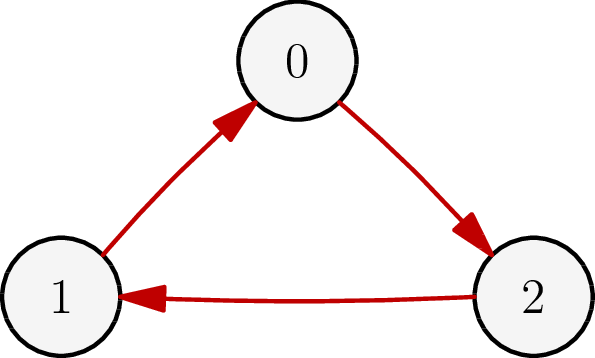
\includegraphics[scale=1]{asy_circuiti/fig1.pdf}
	\vspace{-5pt}
\end{center}
Nel \textbf{terzo caso di esempio}, dato sempre lo stesso input, i valori dei registri saranno:
\begin{multicols}{3}
	$\texttt{somma[0]} = 0$ \\
	$\texttt{somma[12]} = -7$ \\
	$\texttt{somma[23]} = 8$ \\
	$\texttt{somma[123]} = -2$ \\
	$\texttt{mx[0]} = 0$ \\
	$\texttt{mx[1]} = 3$ \\
	$\texttt{mx[2]} = 5$ \\
	$\texttt{mx[3]} = 5$ \\
	$\texttt{mx[4]} = 8$ \\
	$\texttt{out[0]} = 8$ \\
\end{multicols}
\begin{center}
	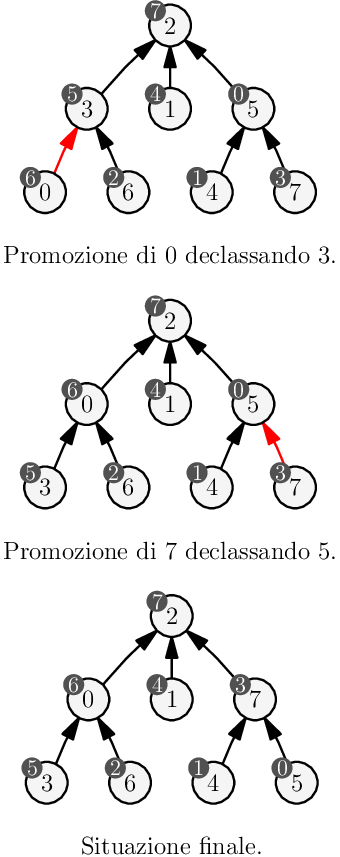
\includegraphics[scale=1]{asy_circuiti/fig2.pdf}
\end{center}
